% UICTEST.TEX
% This is a test file for my port of UICTHESI
% to LaTeX 2e. This is based in part on UCTHESIS.
%

\documentclass{uicthesi}




\usepackage{booktabs} % For formal tables

\usepackage{framed}
\usepackage{hyperref}
\usepackage{balance}
\usepackage[dvips]{graphics,color}

\usepackage{epsfig}
\usepackage{color}
\usepackage{subfigure}
\usepackage{multirow,tabularx}
\usepackage{placeins}
%\usepackage{miniltx}
\usepackage{mathtools}
\usepackage{graphicx}
\usepackage{epstopdf}
\usepackage{bm}

\usepackage{csquotes}
\usepackage{array}
\usepackage[yyyymmdd,hhmmss]{datetime}
\usepackage[subject={Todo}]{pdfcomment}
\usepackage[textsize=scriptsize,bordercolor=black!20]{todonotes}
\usepackage{xcolor,colortbl}
\usepackage{amssymb}% http://ctan.org/pkg/amssymb
\usepackage{pifont}% http://ctan.org/pkg/pifont
\usepackage[algo2e,titlenumbered,ruled]{algorithm2e} 
\usepackage{lipsum,environ,amsmath}
\usepackage{slashbox,booktabs,amsmath}
%\usepackage{todonotes}
\usepackage{cite}


\usepackage{dsfont}
\usepackage{amsfonts}
\usepackage{comment}

\usepackage{xspace}

\hyphenation{PageRank Convex dictatorship Dic-ta-tor-ship}

\newcounter{Lcount}
\newcommand{\numsquishlist}{
   \begin{list}{\arabic{Lcount}. }
    { \usecounter{Lcount}
 \setlength{\itemsep}{-.1ex}      \setlength{\parsep}{0ex}
      \setlength{\topsep}{0ex}       \setlength{\partopsep}{0ex}
      \setlength{\leftmargin}{1em} \setlength{\labelwidth}{1em}
      \setlength{\labelsep}{0.1em} } }
\newcommand{\numsquishend}{\end{list}}

\newcommand{\squishlist}{
   \begin{list}{$\bullet$}
    { \setlength{\itemsep}{-.1ex}      \setlength{\parsep}{0ex}
      \setlength{\topsep}{0ex}       \setlength{\partopsep}{0ex}
      \setlength{\leftmargin}{.8em} \setlength{\labelwidth}{1em}
      \setlength{\labelsep}{0.5em} } }
\newcommand{\squishend}{\end{list}}



\makeatletter
\DeclareOldFontCommand{\rm}{\normalfont\rmfamily}{\mathrm}
\DeclareOldFontCommand{\sf}{\normalfont\sffamily}{\mathsf}
\DeclareOldFontCommand{\tt}{\normalfont\ttfamily}{\mathtt}
\DeclareOldFontCommand{\bf}{\normalfont\bfseries}{\mathbf}
\DeclareOldFontCommand{\it}{\normalfont\itshape}{\mathit}
\DeclareOldFontCommand{\sl}{\normalfont\slshape}{\@nomath\sl}
\DeclareOldFontCommand{\sc}{\normalfont\scshape}{\@nomath\sc}
\makeatother


\newcounter{problem}
\newenvironment{problem}[1][htb]
  {\renewcommand{\algorithmcfname}{Problem}% Update algorithm name
   \begin{algorithm2e}[#1]%
   \SetAlFnt{\small}
    \SetAlCapFnt{\small}
    \SetAlCapNameFnt{\small}
    \SetAlCapHSkip{0pt}
  }{\end{algorithm2e}}
  
  \newenvironment{alprocedure}[1][htb]
  {\renewcommand{\algorithmcfname}{Procedure}% Update algorithm name
   \begin{algorithm2e}[#1]%
    \SetAlFnt{\small}
\SetAlCapFnt{\small}
\SetAlCapNameFnt{\small}
\SetAlCapHSkip{0pt}
\IncMargin{-\parindent}
   
  }{\end{algorithm2e}}
  


\begin{document}

% Declarations for Front Matter

\title{Title of Thesis is here}
\author{Thiruvenkadam Sivaprakasam Radhakrishnan}
\pdegrees{}
\degree{Master's in Computer Science}
\committee{Prof. Firstname1 Lastname1, Chair and Advisor \\ Prof. Firstname2 Lastname2  \\ Prof. Firstname3 Lastname3 \\ Prof. Firstname4 Lastname4 \\ Prof. Firstname5 Lastname5}
\maketitle


% \dedication
% {\null\vfil
% {\large
% \begin{center}
% To myself,\\\vspace{12pt}
% Perry H. Disdainful,\\\vspace{12pt}
% the only person worthy of my company.
% \end{center}}
% \vfil\null}


 \acknowledgements
{The thesis has been completed... (INSERT YOUR TEXTS)\\ 

\begin{flushright}YOUR INITIAL\end{flushright}}
% \acknowledgements
% {I want to ``thank'' my committee, without whose ridiculous demands, I
% would have graduated so, so, very much faster.}

% \preface
% This preface is purely optional at UIC.

\tableofcontents
\listoftables
\listoffigures
\listofabbreviations
\begin{list}
{}
{\setlength
  {\labelwidth}{1in}
    \setlength{\leftmargin}{1.5in}
    \setlength{\labelsep}{.5in}
    \setlength{\rightmargin}{\leftmargin}}
\item[AMS\hfill] American Mathematical Society
\item[CTAN\hfill] Comprehensive \TeX\ Archive Network
\item[TUG\hfill] \TeX\ Users Group
\item[UIC\hfill] University of Illinois at Chicago
\item[UICTHESI\hfill] Thesis formatting system for use at UIC.
\end{list}
 
\summary
Put your summary of thesis here.

Things to add:

\begin{enumerate}
  \item Online Learning and Online Convex optimization
    \begin{enumerate}
      \item General intro
      \item FoReL
      \item Mirror Descent
      \item Hedge
      \item Mirror Descent with KL Divergence
    \end{enumerate}
  \item Policy gradients
  \begin{enumerate}
    \item General intro
    \item Actor critic methods
    \item PPO
  \end{enumerate}
  \item NeuRD
  \item Making the connection between Mirror Descent and Policy gradients
  \begin{enumerate}
    \item MDPO
    \item MMD
  \end{enumerate}
  \item NeuRD fix
  \begin{enumerate}
    \item MDPO
    \item MMD
  \end{enumerate}  
  \item Experiments
  \begin{enumerate}
    \item Rock paper scissors; Khun Poker
    \item MDPO vs MDPO-NR
    \item MMD vs MMD-NR
  \end{enumerate}
\end{enumerate}



\newtheorem{theorem}{Theorem}


\chapter{Derivations}

\section{Online Learning}


\subsection{FoReL}


\section{Online Mirror Descent}


The FoReL update rule is,

\begin{align*}
    w_{t+1} &= argmin_w R(w) + \sum_{i=1}^t \langle w, z_t \rangle \\
            &= argmin_w R(w) + \langle w, z_{1:t}\rangle \\
            &= argmax_w \langle w, -z_{1:t} \rangle - R(w)    
\end{align*}

Let $g(\theta) = argmax_w \langle w, \theta \rangle - R(w)$. Then the FoReL update rule can 
be written as,

\begin{align*}
    \theta_{t+1} = \theta_t - z_t
    w_{t+1} = g(\theta_{t+1})
\end{align*}

where $g(\theta)$ is a link function that projects the predictions back to the convex set $S$.

Using different regularization functions yield different algorithms that have different regret bounds.

\begin{theorem}
    If R is a $(\frac{1}{\eta})$-strongly-convex function over $S$ with respect to some norm $\|.\|$, and OMD 
    is run on a sequence with the following link function

    $$g(\theta) = argmax_w (\langle w, \theta \rangle - R(w))$$

    then,

    $$\forall u \in S, Regret_T(u) \leq R(u) - min_{v \in S} R(v) + \eta \sum_{t=1}^T \|z\|_*^2$$

    where $\|.\|_*$ is the dual norm.
\end{theorem}


\subsection{Hedge}


Hedge or normalized Exponentiated Gradient is OMD with entropic regularization. The link function here is

\begin{equation}
    g_i(\theta) = \frac{e^{\eta \theta[i]}}{\sum_j e^{\eta \theta[j]}}.
\end{equation}

Fitting this into the OMD framework yields the following update rule,

\begin{align*}
    w_{t+1}[i] = \frac{w_t[i] e^{-\eta z_t[i]}}{\sum_j w_t[j] e^{-\eta z_t[j]}}
\end{align*}

We can analyze the regret bounds of Hedge with $R(w) = \frac{1}{\eta} \sum_i w[i] log(w[i])$. 


It is also useful to analyze OMD with the language of duality. The framework utilizing duality makes it easier 
in deriving new algorithms and also in proving tighter regret bounds.

\subsection{Fenchel Conjugacy}

The Fenchel conjugate of a function $f$ is defined as,

$$f^*(\theta) = max_u \langle u, \theta \rangle - f(u)$$

Fenchel conjugate by definition implies the Fenchel-Young inequality:

$$\forall u, f^*(\theta) \geq \langle u, \theta \rangle - f(u)$$.

If $u$ is a sub-gradient of $f^*$ at $\theta$ and if $f^*$ is differentiable, then the equality 
condition holds when $u = \nabla f^*(\theta)$. 


\subsection{Bergman Divergences}

For a differentiable function $R$, the Bergman divergence between two vectors is defined as,

\begin{equation}
    D_R(w \| u) = R(w) - R(u) + (\langle R(u), w-u \rangle)
\end{equation}

Bergman divergence is asymmetric and is always non-negative if R is convex.

\subsection{Online Mirror Descent in terms of Duality}

The link function in the OMD framework is defined as,

$$g(\theta) = argmax_w (\langle w, \theta \rangle - R(w)).$$

This can be also rewritten in terms of the conjugate of $R$ as,

$$g(\theta) = \nabla R^*(\theta)$$

With this, we can obtain different algorithms by using different regularization functions and deriving 
the update rules by using their conjugate.

\subsection{KL-Divergence and its Fenchel Conjugate}

KL-Divergence is a distance metric between two probability distributions and is defined as,

$$D_{KL}(p \| q) = \sum_i p[i] log \frac{p[i]}{q[i]}$$


% TODO: Derivation of the fenchel conjugate
The Fenchel Conjugate of KL-Divergence is given by,

$$f^*_q(x) = \log (\sum_i q_i e^{x_i}).$$


\section{MDPO}

The on-policy MDPO update rule is written as,

$$\theta_{k+1} \leftarrow argmax_{\theta \in \Theta} \Psi(\theta, \theta_k)$$

where,

$$\Psi(\theta, \theta_k) = \mathbb{E}_{s \sim \rho_{\theta_{k}}} [\mathbb{E}_{a \sim \pi_{\theta}}[A^{\theta_k}(s, a)] - \frac{1}{t_k} KL(s; \pi_{\theta}, \pi_{\theta_k})]$$


The gradient of the above update rule is as follows:

\begin{align*}
    \nabla_{\theta} \Psi(\theta, \theta_k) |_{\theta=\theta_k}
                                    &= \mathbb{E}_{s \sim \rho_{\theta_k}} [\sum_a \nabla_{\theta} \pi_{\theta} (a|s) A^{\theta_k}(s, a)] \\
                                    &= \mathbb{E}_{s \sim \rho_{\theta_k}} [\sum_a \pi_{\theta_k}(a|s) \frac{\nabla_{\theta} \pi_{\theta}(a|s)}{\pi_{\theta_k}(a|s)}  A^{\theta_k}(s, a)] \\
                                    &= \mathbb{E}_{s \sim \rho_{\theta_k}, a \sim \pi_{\theta_k}} [\nabla \log \pi_{\theta_k} (a|s) A^{\theta_k}(s,a)]
\end{align*}

For one-step MDPO, the gradient of the KL-Divergence term becomes 0. Hence it is proposed that the policy update at each iteration $k$ is done through $m$ steps of SGD.

$${\theta_k^{(0)} = \theta_k},$$

$$\theta_k^{(i+1)} \leftarrow \theta_k^{(i)} + \eta \nabla_{\theta} \Psi(\theta, \theta_k)|_{\theta=\theta_k^{(i)}}$$

and, $\theta_{k+1} = \theta_k^{(m)}$.


Then the gradient of the objective function evaluated at each step of the SGD update is,

\begin{align*}
    \nabla_{\theta} \Psi(\theta, \theta_k)|_{\theta = \theta_k^{(i)}} &=
                    \mathbb{E}_{s \sim \rho_{\theta_k}, a \sim \pi_{\theta_k}}[\frac{\pi_{\theta_k}^{(i)}}{\pi_{\theta_k}} \nabla \log \pi_{\theta_k^{(i)}} (a|s) A^{\theta_k}(s,a)] \\
                    &- \frac{1}{t_k} \mathbb{E}_{s \sim \rho_{\theta_k}}[\nabla_{\theta} KL(s; \pi_{\theta}, \pi_{\theta_k})|_{\theta = \theta_k^{(i)}}].
\end{align*}


$$KL(s; \pi_{\theta}, \pi_{\theta_k}) = \sum_{a \in \mathcal{A}} \pi_{\theta_k^{(i)}}(a|s) \log \frac{\pi_{\theta_k^{(i)}}(a|s)}{\pi_{\theta_k}(a|s)}$$

The gradient of the KL-Divergence term is given by,

\begin{align*}
    \nabla_{\theta} KL(s; \pi_{\theta}, \pi_{\theta_{k}})|_{\theta = \theta_{k}^{(i)}} 
    &= \sum_{a \in \mathcal{A}} [\nabla_{\theta_{k}^{(i)}} (\pi_{\theta_k^{(i)}}(a|s) \log \pi_{\theta_k}^{(i)}(a|s)) - \nabla_{\theta_k^{(i)}} (\pi_{\theta_k^{(i)}}(a|s) \log \pi_{\theta_k}(a|s))] \\
    &= \log \pi_{\theta_k^{(i)}}(a|s) \nabla_{\theta_{k}^{(i)}} \pi_{\theta_k^{(i)}}(a|s) + \nabla_{\theta_{k}^{(i)}} \pi_{\theta_k^{(i)}}(a|s) - \log \pi_{\theta_{k}}(a|s) \nabla_{\theta_{k}^{(i)}} \pi_{\theta_{k}^{(i)}}(a|s)\\
    &= \sum_{a \in \mathcal{A}} [(\log \pi_{\theta_{k}}^{(i)}(a|s) + 1 - \log \pi_{\theta_k}(a|s)) \nabla_{\theta_{k}^{(i)}}{\pi_{\theta_k^{(i)}}}(a|s)].
\end{align*}



As for the first term of the gradient, it can be seen that the gradient includes a term to account for the fact that the action $a$ was sampled from the policy $\pi_{\theta_k}$

\begin{align*}
    \nabla_{\theta} \Psi(\theta, \theta_k)|_{\theta = \theta_k^{(i)}}
        &= \mathbb{E}_{s \sim \rho_{\theta_k}} [\sum_a \nabla_{\theta_k^{(i)}} \pi_{\theta_k^{(i)}}(a|s) A^{\theta_k}(s, a)] \\
        &= \mathbb{E}_{s \sim \rho_{\theta_k}} [\sum_a \pi_{\theta_k}(a|s) \frac{\pi_{\theta_k^{(i)}}(a|s)}{\pi_{\theta_k}(a|s)} \frac{\nabla_{\theta_k^{(i)}} \pi_{\theta_k^{(i)}}(a | s)}{\pi_{\theta_k^{(i)}}(a|s)} A^{\theta_k}(s, a)] \\
        &= \mathbb{E}_{s \sim \rho_{\theta_k}, a \sim \pi_{\theta_k}} [\frac{\pi_{\theta_k^{(i)}}(a|s)}{\pi_{\theta_k}(a|s)} \nabla_{\theta_k^{(i)}} \log \pi_{\theta_k^{(i)}}(a | s) A^{\theta_k}(s, a)]
\end{align*}



































































%\documentclass{article}

%\usepackage{dsfont}
%\usepackage{amsfonts}

%\begin{document}

%\title{Derivations for the main thesis}

\newtheorem{definition}{Definition}
\newtheorem{lemma}{Lemma}

\chapter{Online Learning and Online Convex Optimization}

\section{Online Learning}

Online Learning is a sub-domain of machine learning that has important theoretical and practical applications. 
In Online Learning, a learner is tasked with predicting the answer to a set of questions over a sequence of consecutive rounds.
At each round t, a question $x_t$ is taken from an instance domain $\mathcal{X}$, and the learner is required to predict 
an answer, $p_t$ to this question. After the prediction is made, the correct answer $y_t$, from a target domain $\mathcal{Y}$ 
is revealed and the learner suffers a loss $l(p_t, y_t)$. The prediction $p_t$ could belong to $\mathcal{Y}$ or a larger set, 
$\mathcal{D}$.

There are many special cases of Online learning that translate to popular Online learning problems. Some common ones are,

Online Classification: $\mathcal{Y}=\mathcal{D}=\{0,1\}$, and typically the loss function is the 0-1 loss: $l(p_t, y_t)=|p_t - y_t|$.

Online Regression:

Expert's case:


The goal of an Online learning algorithm is to minimize the cumulative loss across all the rounds it has been through so far.
The learner uses the information from the previous rounds to improve its prediction on present and future rounds.

The sequence of questions can be deterministic, stochastic or even adversarial. This means, for any online learning algorithm 
an adversary can make the cumulative loss unbounded, by simply providing an opposing answer to the algorithm's answer as the correct 
answer. To make learning possible, certain restrictions are imposed on the structure of the problem.

Realizability: It is assumed that the answers are generated by a target mapping $h^*: \mathcal{X} \rightarrow \mathcal{Y}$, and that $h^*$ is 
taken from a fixed set, $\mathcal{H}$ called the hypothesis class. Now, for any Online learning algorithm, A, $M_A(\mathcal{H})$ is the number 
of mistakes $A$ makes on a sequence of questions, labelled by some $h^* \in \mathcal{H}$. $M_A(\mathcal{H})$ is called the $\textit{mistake-bound}$ 
of $A$.

A relaxation from realizable assumption is that the answers are not generated by some fixed mapping $h^*$, but the learner is still only required 
to be competitive with the best fixed predictor from $\mathcal{H}$. This is the regret of an Online learning algorithm for not having followed a 
fixed hypothesis $h^* \in \mathcal{H}$.

\begin{equation}\label{eqn_regretdef}
    Regret_T(h^*) = \sum_{t=1}^T l(p_t, y_t) - \sum_{t=1}^T l(h^*(x_t), y_t),
\end{equation}

The regret of $A$ with $\mathcal{H}$ is,

\begin{equation}\label{eqn_regretdef}
    Regret_T(\mathcal{H}) = max_{h^* \in \mathcal{H}} Regret_T(h^*)
\end{equation}


\section{Online Convex Optimization}

An established approach to design efficient online learning algorithm has been using convex optimization. This typically frames online learning as an 
online convex optimization problem as follows:

input: a convex set S
for t = 1, 2. $\ldots$
predict a vector $w_t \in S$
receive a convex loss function $f_t: S \mapsto \mathbb{R}$

Reframing \ref{eqn_regretdef} in terms of convex optimization, we refer to a competing hypothesis here as some vector $u$ from the convex set $S$.

\begin{equation}
    Regret_T(u) = \sum_{t=1}^T f_t(w_t) - \sum_{t=1}^T f_t(u)
\end{equation}

and similarly, the regret with respect to a set of competing vectors $U$ is,
\begin{equation}
    Regret_T(U) = max_{u \in U} Regret_T(u)
\end{equation}

As stated in the case of online learning, the set $U$ can be same as $S$ or different in other cases. In this work, the default setting is $U=S$ and 
$S=\mathbb{R^d}$ unless specified otherwise.

% Convexification can be added here briefly

\subsection{FoReL}

Follow-the-Regularized-leader (FoReL) is a classic learning algorithm for online convex optimization, where the algorithm tries to minimize the loss on 
all past rounds along with a regularization term. The regularization term is used to stabilize the solution and prevent it from oscillating too much every 
round preventing converging to a solution.

The learning rule can be written as,

$$\forall t, w_t = argmin_{w \in S} \sum_{i=1}^{t-1} f_i(w) + R(w).$$

where $R(w)$ is the regularization term. Different regularization functions lead to different algorithms with varying regret bounds.


In the case of linear loss functions with respect to some $z_t$, i.e., $f_t(w) = \langle w, z_t \rangle$, and $S=\mathbb{R}^d$,  if FoReL is run with 
$l_2$-norm regularization $R(w) = \frac{1}{2 \eta} \|w\|_2^2$ , then the learning rule can be written as,

\begin{equation}
    w_{t+1} = -\eta \sum_{i=1}^t z_i = w_t - \eta z_t
\end{equation}

Since, $\nabla f_t(w_t) = z_t$, this can also be written as, $w_{t+1} = w_t - \eta \nabla f_t(w_t)$. This update rule is also commonly known as Online Gradient Descent.
The regret of FoReL run on Online linear optimization with a euclidean-norm regularizer is:

$$Regret_T(U) \leq BL \sqrt {2T}.$$

where $U = {u : \|u\| \leq B}$ and $\frac{1}{T} \sum_{t=1}^T \|z_t\|_2^2 \leq L^2$ with $\eta = \frac{B}{L\sqrt{2T}}$.

This can also be generalized to Convex Functions in general through linearization using the property of convex functions. For a convex set S, a convex function $f: S \mapsto \mathbb{R}$ is convex iff $\forall w \in S, \exists z$ such that,

\begin{equation}
    \forall u \in S, f(u) \leq f(w) + \langle u-w, z \rangle  
\end{equation}

Following this, in Online Convex Optimization for each round $t$, there exists a $z_t$ such that for all competing hypothesis $u$, 

$$f_t(w_t) - f_t(u) \leq \langle w_t - u, z_t \rangle.$$

where $z_t \in \partial f_t(w_t)$ is a sub-gradient of $f_t$ at $w_t$.

Then, for a sequence of convex loss functions $f_1, \ldots, f_T$ and vectors $w_1, \ldots, w_T$ and if for all $t$, $z_t \in \partial f_t(w_t)$,

\begin{equation}
    \sum_{t=1}^T (f_t(w_t) - f_t(u)) \leq \sum_{t=1}^T (\langle w_t, z_t\rangle - \langle u, z_t \rangle)
\end{equation}

This implies, the regret of an algorithm for Online Convex Optimization is upper bounded by the regret with respect to the linearization of the 
sequence of convex functions.

% Add details about theorem 2.4 and discuss about the requirement of the norm of z_t to be bounded by L, and how it relates to the lipschitzness of the loss function

Beyond Euclidean regularization, FoReL can also be run with other regularization functions and yield similar regret bounds given that the regularization functions are 
strongly convex.

\begin{definition}
    For any $\sigma$-strongly-convex function $f: S \mapsto \mathbb{R}$ with respect to a norm $\|.\|$, for any $w \in S$,
    \begin{equation}
        \forall z \in \partial f(w), \forall u \in S, f(u) \geq f(w) + \langle z, u - w\rangle + \frac{\sigma}{2}\| u - w \|^2.
    \end{equation}
\end{definition}


% Lemma 2.3 to be shifted above

\begin{lemma}\label{lem:forelrb}
    For a FoReL algorithm producing a sequence of vectors $w_1, \ldots, w_T$ with a sequence of loss functions $f_1, \ldots, f_T$, for all $u \in S$, 
    $$\sum_{t=1}^T (f_t(w_t) - f_t(u)) \leq R(u) - R(w_1) + \sum_{t=1}^T (f_t(w_t) - f_t(w_{t+1}))$$
\end{lemma}

\subsection{FoReL with Strongly Convex Regularizers}
From Lemma \ref{lem:forelrb}, the regret bound is given by,

$$\sum_{t=1}^T (f_t(w_t) - f_t(u)) \leq R(u) - R(w_1) + \sum_{t=1}^T (f_t(w_t) - f_t(w_{t+1}))$$

If $f_t$ is $L$-Lipschitz with respect to some norm $\|.\|$ then,

$$f_t(w_t) - f_t(u) \leq L \| w_t - w_{t+1} \|$$

If $\| w_t - w_{t+1} \|$ is small that leads to a better regret bound. It can be shown that if the regularization function $R(w)$ is strongly convex with 
respect to the same norm $\|.\|$ then $\|w_t - w_{t+1}\|$ is also bounded.

For a sequence of predictions $w_1, w_2, \ldots$ of the FoReL algorithm, with a regularizer $R: S \mapsto \mathbb{R}$,

$$f_t(w_t) - f_t(w_{t+1}) \leq L_t \|w-t - w_{t+1} \| \leq \frac{L_t^2}{\sigma}.$$

if $f_t$ is $L$-Lipschitz with respect to $\|.\|$ and $R$ is $\sigma$-strongly-convex.

\begin{theorem}\label{thm:forelregret}
    FoReL run on a sequence of convex functions $f_1, \ldots, f_T$ such that $f_t$ is $L_t$-Lipschitz, with a $\sigma$-strongly-convex regularization function 
    has a regret bound given by, 

    $$Regret_T(u) \leq R(u) - min_{v \in S} R(v) + \frac{TL^2}{\sigma}$$

    where $\frac{1}{T} \sum_{t=1}^T L_t^2 \leq L^2$.
\end{theorem}

\textcolor{red}{To add: derived regret bounds for euclidean and entropic regularizers}

\section{Online Mirror Descent}




% 

\begin{comment}
Mirror Descent:

Mirror descent with entropy regularization

Mirror descent with KL Divergence regularizations 


Mirror Descent Policy optimization (MDPO)

The update rule for on-policy MDPO is given by,

$\theta_{k+1} \leftarrow argmax_{\theta \in \Theta \psi(\theta, \theta_k)}$

$\psi(\theta, \theta_k) = \mathds{E}_{s ~ \rho_{\theta_k}}[\mathds{E}_{a~\pi_{\theta}}[A^{\theta_k}(S, a)] - \frac{1}{t_k} \textrm{KL}(s; \pi_{\theta}, \pi_{\theta_k})]$

\end{comment}

%\end{document}

\chapter{Introduction}

This is how we cite a paper \cite{Farine20162243}.

Below is the example of algorithm block.


\IncMargin{1em}
\begin{alprocedure}[!htp]
\caption{FindFactionsAndInitiators}
\SetKwInOut{Input}{input}\SetKwInOut{Output}{output}
\Input{An adjacency matrix $E^*$ of dynamic network}
\Output{ A time series of faction sets $\mathcal{F}^*$, and a time series of initiator sets $\mathcal{L}^*$ }
\BlankLine
\For{$i\leftarrow 1$ \KwTo $t^*$}{
\textcolor{cyan}{\tcc*[h]{Get a matrix at time $t=i$} }

$E \leftarrow E^*_{ t = i}$ \; 
\textcolor{cyan}{\tcc*[h]{FindInitiators($E $) returns all nodes which have zero outgoing degree}}

$\mathcal{L} \leftarrow$FindInitiators($E $) \;
$\mathcal{F} = \emptyset$ \;
\For{$l \in \mathcal{L}$}{
\textcolor{cyan}{\tcc*[h]{FindReachNodeFrom($E,l$) returns all nodes which have any directed path to $l$}}

$F_l\leftarrow$FindReachNodeFrom($E,l$) \;
$\mathcal{F} = \mathcal{F} \cup \{F_l\}$
}
$\mathcal{F}^*_{t=i} = \mathcal{F}  $ and $\mathcal{L}^*_{t=i} = \mathcal{L}  $
}
\label{algo:FindFactionsAndInitiators}
\end{alprocedure}\DecMargin{1em}


The example of table is below.

\begin{table}[!htp]
\tiny
\centering
\caption{Table Caption1}
\label{table:htestdes}
\begin{tabular}{l|l|l|}
\cline{2-3}
                                                                                                                     & \cellcolor[HTML]{EFEFEF}\textbf{Method}                                    & \cellcolor[HTML]{EFEFEF}\textbf{Null hypothesis $H_0$}                                                                                          \\ \hline
\multicolumn{1}{|l|}{}                                                                                               & $t$-test                                                                      & \begin{tabular}[c]{@{}l@{}}A sample has a normal distribution \\ with zero mean and unknown variance.\end{tabular}                              \\ \cline{2-3} 
\multicolumn{1}{|l|}{}                                                                                               & \cellcolor[HTML]{EFEFEF}Sign test                                          & \cellcolor[HTML]{EFEFEF}A sample has a distribution with zero median.                                                                           \\ \cline{2-3} 
\multicolumn{1}{|l|}{\multirow{-3}{*}{\textbf{\begin{tabular}[c]{@{}l@{}}Zero \\ mean/median \\ test\end{tabular}}}} & Wilcoxon signed rank test                                                  & A sample has a symmetric distribution around zero median.                                                                                       \\ \hline
\multicolumn{1}{|l|}{}                                                                                               & \cellcolor[HTML]{EFEFEF}Kolmogorov-Smirnov test (KS test)                           & \cellcolor[HTML]{EFEFEF}A sample comes from a normal distribution.                                                                              \\ \cline{2-3} 
\multicolumn{1}{|l|}{}                                                                                               & \begin{tabular}[c]{@{}l@{}}Chi-square \\ goodness-of-fit test\end{tabular} & \begin{tabular}[c]{@{}l@{}}A sample comes from a normal distribution \\ with a mean and variance estimated from a sample itself.\end{tabular}   \\ \cline{2-3} 
\multicolumn{1}{|l|}{}                                                                                               & \cellcolor[HTML]{EFEFEF}Jarque-Bera test                                   & \cellcolor[HTML]{EFEFEF}\begin{tabular}[c]{@{}l@{}}A sample comes from a normal distribution \\ with an unknown mean and variance.\end{tabular} \\ \cline{2-3} 
\multicolumn{1}{|l|}{\multirow{-4}{*}{\textbf{\begin{tabular}[c]{@{}l@{}}Normality \\ test\end{tabular}}}}           & Anderson-Darling test                                                      & A sample comes from a normal distribution.                                                                                                      \\ \hline
\end{tabular}
\end{table}



\section{Support of leading faction}

\begin{figure}[ht!]
\centering
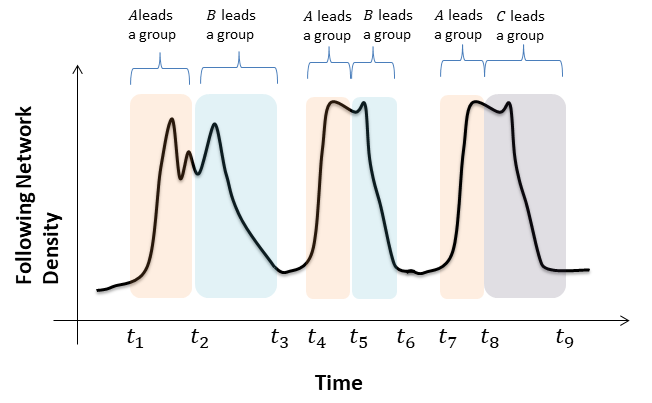
\includegraphics[width=0.9\columnwidth]{FIG/CoorEventSup}
\caption{An example of image in thesis }
\label{fig:CoorEventSup}
\end{figure}


 \appendices
 \newpage
 \appendix

 \chapter{Some Ancillary Stuff}

 Ancillary material should be put in appendices.

 \chapter{Some More Ancillary Stuff}

% Here is yet another appendix! Wahoo!

%\nocite{*}
\bibformb
\bibliography{BibFile}
\newpage
% \vita
% This is where the vita goes.  Its organization is left as an exercise.
\clearpage
    \pagestyle{pageontop}
   \thispagestyle{pageonbottom}
   %\vspace*{3in}
   \begin{large}
   \begin{center}
   {\bfseries VITA}
   \end{center}
   \end{large}
\begin{tabular}{p{2.8cm}p{10.5cm}}
NAME: & NAME LASTNAME  \\ 
    &\\
EDUCATION:  &Ph.D., Computer Science, University of Illinois at Chicago, Chicago, Illinois, 2018. \\  
            &\\
            &M.Eng., Computer Engineering, University of Illinois at Chicago, Chicago, Illinois, 20xx.\\
            &\\
            &B.Eng., Computer Engineering, University of Illinois at Chicago, Chicago, Illinois, 20xx.  \\
            &\\
ACADEMIC EXPERIENCE:  &Research Assistant, Computational Population Biology Lab, Department of Computer Science, University of Illinois at Chicago, xxxx - 2018. \\
            &\\
            &Teaching Assistant, Department of Computer Science, University of Illinois at Chicago: \\
            &\squishlist            
            \item Computer Algorithm I, Spring xxxx and  Fall xxxx.    
            \item Secure Computer Systems, Fall xxxx 
            \squishend \\
            

 \end{tabular}

\end{document}
